Un pequeño pez se encuentra dentro de un acuario. La figura de este ejercicio muestra rayos luminosos que parten del pez y se refractan al pasar del agua hacia el aire.
\begin{enumerate}
    \item Muestre, en la figura, dónde está situada la imagen del pez que ve el observador.
    \item Esta imagen, ¿es real o virtual? Explique.
    \item Si el observador deseara atrapar al pecesillo con un arpón, ¿deberá dirigir el arma hacia un punto situado arriba o abajo de la posición donde ve el pez?
\end{enumerate}
\begin{figure}[h!]
  \centering
  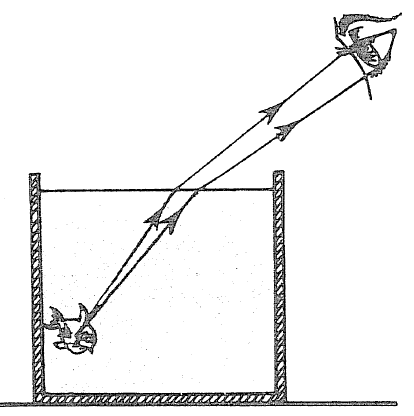
\includegraphics[scale=0.44]{figuras/fig_alvarenga_p671_6.png}
  \caption{Problema 14}
\end{figure}